\section{Wie genau ist der Mittelwert?}
\kopfrechts{Wie genau ist der Mittelwert?}
Der Erwartungswert drückt aus, wie gross eine Zufallvariable ``im Mittel''
sein wird.
Je grösser aber die Varianz ist, desto grösser wird die Abweichung
der Zufallsvariable vom ``mittleren Wert'' sein.
Wie misst man diese Abweichung? Mit der Varianz haben wir bereits
ein Mass für die mittlere Abweichung, aber noch keinen Hinweis
darauf, wie häufig grosse Abweichungen vorkommen werden.

Sei $\mu=E(X)$ der Erwartungswert der Zufallsvariablen $X$.
Für die Varianz hatten wir die Abweichung $X-\mu$ der Zufallsvariablen
von ihrem Erwartungswert untersucht.
Meistens wird die Abweichung klein sein.
Uns interessiert jetzt aber,
wie wahrscheinlich es ist, dass sie gross ist.
Sei $\varepsilon>0$ ein Schwellwert für die Abweichung, wir möchten
also wissen, wie häufig die Abweichung die Schranke $\varepsilon$
überschreitet:
\[
|X-\mu|>\varepsilon,
\]
wir möchten also die Wahrscheinlichkeit 
\[
P(|X-\mu|>\varepsilon)
\]
berechnen.
Nach unseren einleitenden Bemerkungen sollte es einen Zusammenhang
zwischen Varianz und dieser Wahrscheinlichkeit geben: je grösser
die Varianz, desto grösser die Wahrscheinlichkeit einer grossen
Abweichung.

\subsection{Ungleichung von Tschebyscheff} \label{ungleichung-von-tschebyscheff}
\index{Tschebyscheff!Ungleichung von}
Selbst wenn man gar nichts über die Zufallsvariable weiss, ausser
dass sie eine Varianz besitzt, kann man eine Aussage über die 
Wahrscheinlichkeit einer grossen Abweichung machen.
Dies ist der Inhalt der Ungleichung von Tschebyscheff.
Dies kann natürlich
nur eine grobe obere Schranke sein, für genaue Resultate muss man
mehr über das konkrete Experiment wissen.
\begin{figure}
\centering
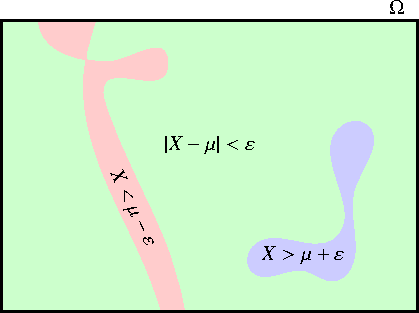
\includegraphics{images/erwartung-5.pdf}
\caption{Zur Herleitung der Tschebyscheff-Ungleichung: Ereignisse, in denen 
die Zufallsvariable um mehr als $\varepsilon$ vom Erwartungswert $\mu$
abweicht.
\label{tschebyscheff-herleitung}}
\end{figure}
\begin{figure}
\centering
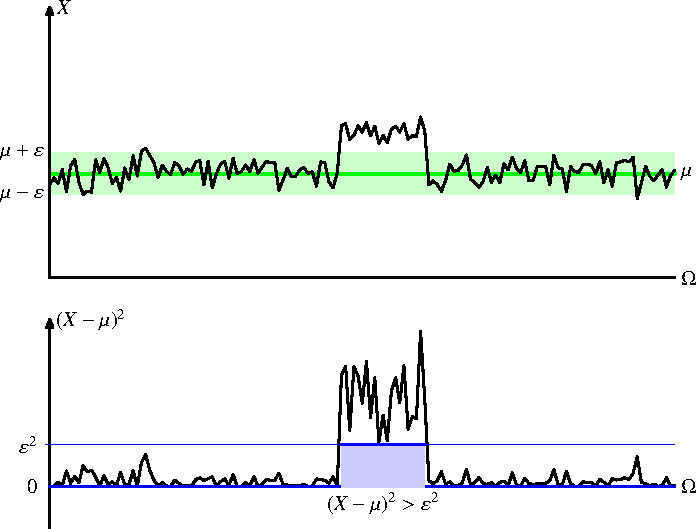
\includegraphics{images/erwartung-6.pdf}
\caption{Herleitung der Tschebyscheff-Ungleichung, charakteristische Funktion
des Ereignisses $|X-\mu|>\varepsilon$ ist blau eingezeichnet.
\label{tschebyscheff2}}
\end{figure}

\begin{satz}[Ungleichung von Tschebyscheff]
Ist eine Zufallsvariable $X$, dann lässt sich die Wahrscheinlichkeit,
dass $X$ um mehr als $\varepsilon$ vom Erwartungswert abweicht, wie
folgt abschätzen:
\[
P(|X-\mu| >\varepsilon)\le\frac{\operatorname{var}(X)}{\varepsilon^2}.
\]
\end{satz}

Lässt man $\varepsilon$ wachsen findet man, dass Abweichungen
deutlich grösser als $\sqrt{\operatorname{var}(X)}$ 
sehr unwahrscheinlich sind.

\begin{proof}[Beweis]
Sei $A =\{\omega\;|\;|X(\omega)-\mu|>\varepsilon\}$ das Ereignis, dass die
Zufallsvariable $X$ um mehr als $\varepsilon$ vom Mittelwert abgewichen
ist.
Dies ist in Abbildung~\ref{tschebyscheff-herleitung} das rote und blaue Gebiet.
Offensichtlich ist dies dasselbe, wie wenn $(X-\mu)^2$ mehr als
$\varepsilon^2$ von 0 abweicht.
Es gilt daher:
\[
\varepsilon^2 \chi_{A} \le (X-\mu)^2,
\]
wie man auch aus der Abbildung~\ref{tschebyscheff2} ablesen kann.
Wenden wir darauf den Erwartungswert an, folgt
\[
\varepsilon^2 P(A)\le E((X-\mu)^2)=\operatorname{var}(X)
\]
Die Tschebyscheffsche Ungleichung folgt jetzt nach Division durch
$\varepsilon^2$.
\end{proof}
Beispiel:
Bei der Herstellung von 1k$\Omega$ Widerständen
möchte man sicherstellen,
dass nur bei 1\% aller produzierten Widerstände der Wert um mehr als
10$\Omega$ vom Sollwert abweicht.
Um das zu überprüfen entnimmt man der
Produktion eine Stichprobe, und schätzt die Varianz ab.
Wie gross darf die
Varianz maximal werden, damit die Bedingung noch erfüllt ist?

Die Tschebyscheffsche Ungleichung liefert in diesem Fall
\[
\operatorname{var}(X)\ge\varepsilon^2P(|X-\mu| >\varepsilon)
\]
oder
\[
\operatorname{var}(X)\ge 10^2\cdot 0.01=1.
\]
Sobald die Varianz der Stichprobe grösser als 1$\Omega^2$ ist, kann die
Tschebyscheffungleichung die Einhaltung der Qualitätsvorgabe nicht
mehr garantieren.

Die Tschebyscheff-Ungleichung ist bei weitem nicht die bestmögliche.
Fragt man zum Beispiel nach der Wahrscheinlichkeit, dass $X$ um mehr
als zwei Standardabweichungen, also um mehr als $2\sqrt{\operatorname{var}(X)}$ vom
Erwartungswert abweicht, dann liefert sie
\[
P(|X-\mu|>2\sqrt{\operatorname{var}(X)})
\le\frac{\operatorname{var}(X)}{2^2\operatorname{var}(X)}=\frac14.
\]
Diese Ungleichung gilt für jede Zufallsvariable $X$.
Es gibt aber Zufallsvariablen, für die 
\[
P(|X-\mu|>2\sqrt{\operatorname{var}(X)})\le 0.05.
\]
Wir werden mit der Normalverteilung solche Zufallsvariablen kennenlernen.
Auf das Beispiel angewendet bedeutet dies, dass die Tschebyscheff-Ungleichung
möglicherweise viel zu oft behauptet, dass die Produktionsqualität ungenügend
ist, weil die Widerstandswerte vermutlich in guter Näherung normalverteilt
sein werden.

\subsection{Wie gut approximiert der Mittelwert den Erwartungswert?} \label{approximation-mittelwert}
Wir betrachten eine Folge von unabhängigen Zufallsvariablen $X_1, X_2,\dots$, die
alle den gleichen Erwartungswert $E(X_i)=\mu$ und die gleiche Varianz
$\operatorname{var}(X_i)=\sigma^2$ haben.
Dann erwartet man, dass 
der Mittelwert der ersten $n$ Zufallsvariablen, also die
Grösse
\[
M_n=\frac{X_1+X_2+\dots+X_n}{n}
\]
eine gute Näherung ist für $\mu$. Trotzdem kann es vorkommen, dass wegen
einzelner Ausreisser unter den $X_i$ der Mittelwert recht weit weg
vom Erwartungswert liegt.
Der folgende Satz von Bernoulli sagt, wie wahrscheinlich
es ist, dass der Mittelwert weiter als $\varepsilon$ vom Erwartungswert
entfernt ist.

Zunächst halten wir fest, dass
\[
M_n=\frac{X_1+\dots+X_n}{n}
\]
eine Zufallsvariable ist mit Erwartungswert
\[
E(M_n)=E\biggl(\frac{X_1+\dots+X_n}{n}\biggr)
=\frac{E(X_1)+\dots+E(X_n)}{n}=\mu
\]
und Varianz
\[
\operatorname{var}(M_n) =\frac1{n^2}\sum_{i=1}^n\operatorname{var}(X_i)
=\frac{\sigma^2}n,
\]
wie man mit den Rechenregeln für die Varianz sofort nachrechnet.

\index{Gesetz der grossen Zahlen}
\index{Bernoulli!Gesetz der grossen Zahlen}
\begin{satz}[Bernoullis Gesetz der grossen Zahlen]
Die Wahrscheinlichkeit, dass der Mittelwert von $n$ unabhängigen Zufallsvariablen
mit Erwartungswert $\mu$ und Varianz $\sigma^2$ mehr als $\varepsilon$ von $\mu$
abweicht, ist
\[
P(|M_n-\mu|>\varepsilon)\le \frac{\sigma^2}{\varepsilon^2n}.
\]
Insbesondere gilt
\[
\lim_{n\to\infty}P(|M_n-\mu|>\varepsilon)=0.
\]
\end{satz}
\begin{proof}[Beweis]
Aus der Tschebyscheffschen Ungleichung folgt:
\[
P(|M_n-\mu|>\varepsilon)\le\frac{\operatorname{var}(M_n)}{\varepsilon^2}=
\frac{\sigma^2}{n\varepsilon^2}.
\]
Dies entspricht genau der Behauptung.
\end{proof}
Leider sind die Vorhersagen wie auch bei der Tschebyscheff-Ungleichung
nur beschränkt nützlich.
Wenn die Wahrscheinlichkeit, dass der Mittelwert
um mehr als $\sigma$ vom Erwartungswert abweicht, kleiner als 1\% sein
soll, sind dafür nach dem Gesetz der grossen Zahlen mindestens 100 Summanden
nötig.

\subsection{Wie genau ist die empirische Häufigkeit?}
Wir haben durch Wiederholung von Experimenten auch versucht, die
Wahrscheinlichkeit eines Ereignisses durch die Häufigkeit zu approximieren,
mit welcher dieses Ereignis eintritt.
Mit dem Satz von Bernoulli ist es uns jetzt auch möglich, die
Wahrscheinlichkeit dafür abzuschätzen, dass wir ein falsches
Resultat erhalten.
\begin{satz}
Wird ein Experiment $n$ mal durchgeführt, und tritt dabei das Ereignis $A$
mit der relativen Häufigkeit $h$ ein, dann ist die Wahrscheinlichkeit,
dass $h$ um mehr als $\varepsilon$ von $P(A)$ abweicht
\[
P(|h- P(A)|>\varepsilon)\le \frac{P(A)(1-P(A))}{n\varepsilon^2}
\le\frac{1}{4n\varepsilon^2}.
\]
\end{satz}
\begin{proof}[Beweis]
Wir betrachten die Zufallsvariablen $X_i$, welche den Wert $1$ hat,
wenn im $i$-ten Versuch das Ereignis $A$ eingetreten ist, und sonst $0$.
Diese Zufallsvariablen sind offensichtlich unabhängig.
Betrachtet man
nur die einzelne Durchführung $i$ des Versuches, dann ist $X_i$
die Funktion
$\chi_A$, welchen
den Erwartungswert $E(\chi_A)=P(A)$, und die Varianz ist
\begin{align*}
\operatorname{var}(\chi_A)&=E(\chi_A^2)-E(\chi_A)^2=E(\chi_A)-E(\chi_A)^2\\
&=P(A)-P(A)^2=P(A)(1-P(A))
\end{align*}
hat.
Der Mittelwert $M_n$ ist die Anzahl der Versuche, bei denen das Ereignis
$A$ eingetreten ist, geteilt durch $n$, also die Anzahl aller Versuche,
$h=M_n$.
Damit folgt aus dem Gesetz der grossen Zahlen:
\[
P(|h-P(A)|>\varepsilon)\le\frac{P(A)(1-P(A))}{n\varepsilon^2}.
\]
Die letzte Ungleichung des Satzes folgt aus der Tatsache, dass die Funktion
$p\mapsto p(1-p)=p-p^2$ bei $p=\frac12$ ein Maximum hat, also
$P(A)(1-P(A))\le\frac14$ gilt.
\end{proof}

Insbesondere verstehen wir jetzt, warum es sehr lange dauern kann, bis
wir durch Zählen der Häufigkeit eines Ereignisses dessen Wahrscheinlichkeit
auch nur auf wenige Stellen nach dem Komma bestimmen können.
Wenn wir verlangen, dass die relative Häufigkeit mit
99\% Sicherheit die Wahrscheinlichkeit auf drei Stellen annähert, also
$\varepsilon=10^{-3}$, dann müssen wir verlangen
\begin{align*}
\frac{1}{4n\varepsilon^2}&\le 0.01\\
\frac1{4\cdot 10^{-3\cdot 2}\cdot10^{-2}}=25\cdot 10^6&\le n.
\end{align*}
Der Versuch muss also mindestens 25 Millionen mal wiederholt werden,
um eine Genauigkeit von drei Stellen nach dem Komma mit 99\% Sicherheit
zu erreichen.
Dies deckt sich mit den Beobachtungen in der Würfelsimulation
in Tabelle
\ref{wuerfel-simulation}.
\begin{figure}
\centering
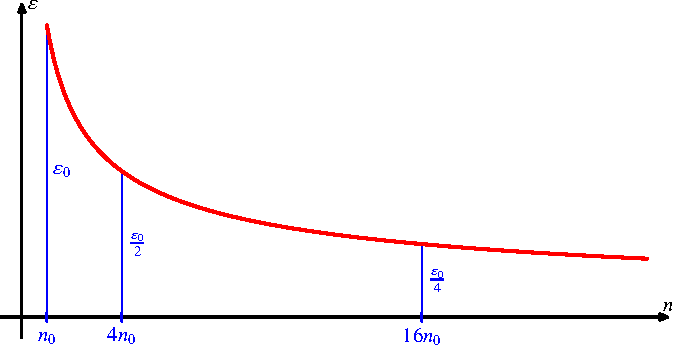
\includegraphics{images/erwartung-7.pdf}
\caption{Abnahme des Fehlers der relativen Häufigkeit mit der Anzahl
Wiederholungen.
Um den Fehler zu halbieren, muss die Anzahl der Versuche
vervierfacht werden.
\label{fehlerabnahme}}
\end{figure}
Der verbleibende Fehler der relativen Häufigkeit ist proportional zu
$\frac1{\sqrt{n}}$, wenn $n$ die Anzahl der Versuche ist.
Die Abhängigkeit des zu erwartenden Fehlers der relativen Häufigkeit mit
der Anzahl der Versuche ist in Abbildung~\ref{fehlerabnahme} dargestellt.


